\chapter{مقدمه}\label{chap1}
\section{معرفی}
از زمانی که گام‌های اوّلیّه در اپتیک نوین برداشته شده تا هم/ اکنون، برهم‌کنش نور و ماده\LTRfootnote{light-matter interaction} نقشی محوری در تحقیقات داشته است~\cite{FriskKockum2019} و در این میان، تابشگر‌ها و کنترل آن‌ها بسیار مورد توجه محققان است.
با مطرح شدن تحقیقات \lr{Purcell} و بیان این نتیجه که «رفتار یک تابشگر، به شدت تحت تأثیر میدان الکترومغناطیس پیرامون آن است»~\cite{Purcell1995,Pelton2015}، تحقیقات روی برهم‌کنش تابشگر و میدان الکترومغناطیس موضوع بسیاری از تحقیقات را به خود اختصاص داده است. تا کنون، تحقیقات بسیاری نشان داده است که هم \emph{توان تابش}~\cite{russell2012large} و هم \emph{نرخ گذار}~\cite{geddes2005radiative} تابشگرها را می‌توان با تنظیم میدان‌های خارجی، به خوبی کنترل کرد.

امّا تنظیم میدان الکترومغناطیس در نزدیکی مولکول و در مقیاس‌های نانومتری خود نیازمند پیش‌زمینه‌های دانش و فناوری است. روش‌هایی که تاکنون برای این منظور مورد استفاده قرار گرفته‌اند محدوده وسیعی از اپتیک نانومتری را در بر می‌گیرد؛ از بلورهای فوتونی~\cite{PhysRevLett.95.013904,Koenderink:05,doi:10.1021/acs.nanolett.7b05075} تا ساختارها و نانوذرات پلاسمونی~\cite{PhysRevLett.89.117401,ribeiro2017artefact}، و اخیرًا ساختارهای دوگانه فوتونی-پلاسمونی (\lr{HPPS})\RTLfootnote{hybrid photonic-plasmonic structures}~\cite{shi2014coherent}.

با توسعه ابزار محاسبات عددی، روش‌های شبیه‌سازی به دلیل هزینه مناسب‌تر و قابلیّت بیشتر برای اعمال شرائط کنترل‌شده و حل مسائل متنوع در مقایسه با آزمایش‌های عملی، به شدّت مورد استقبال محققان قرار گرفته‌ است. از این‌رو، بخش قابل توجهی از تحقیقات نیز متوجه ایجاد، توسعه و تکمیل روش‌های عددی شبیه‌سازی مسائل فیزیکی شده است.
آن‌چنان که در طی این رساله خواهد آمد، روش‌های شبیه‌سازی حاضر در موضوع برهم‌کنش تابشگرها و میدان الکترومغناطیس، علی‌رغم کاربرد فراوان در تحقیقات، نواقص جدی و مهمی دارند و توسعه و بهبود این روش‌ها کمتر مورد توجه قرار گرفته است.

در تحقیق حاضر، اوّلًا، با تعمق در پایه‌های فیزیکی تابش فلورسانس و به صورت کلی‌تر تابش خودبه‌خودی، به معرفی روش مناسبی برای شبیه‌سازی رفتار مولکول‌های تابشگر در حضور میدان الکترومغناطیس  می‌پردازیم و با تطبیق نتائج شبیه‌سازی و نتائج گزارش شده حاصل از آزمایش‌های عملی، کارایی و توان‌مندی روش پیش‌نهادی را بررسی خواهیم کرد.

ثانیًا، با استفاده از روش عددی پیش‌نهادی،‌ ساختار \lr{HPPS} جدیدی را معرفی و بررسی خواهیم کرد که تأثیر ویژه‌ای در بهبود تابش فلورسانس خواهد داشت. این تأثیر ورای تنظیم نرخ گذار یا شدت تابش، منجر به بروز تابشی با همدوسی زمانی و فضایی قابل توجّه از تابشگر‌های خودبه‌خودی خواهد شد.

پیش‌ از ارائه بخش‌های اصلی تحقیق، لازم است مروری بر برخی مطالب فیزیکی و همچنین تحقیقات پیشین انجام گیرد که در ادامه این فصل خواهد آمد.

\section{تابش فلورسانس}
استفاده از تابش فلورسانس یکی از پر کاربردترین ابزارها در بررسی‌های شیمیایی و بیولوژی می‌باشد~\cite{Shcheslavskiy:18,giljohann2009}. دامنه کاربرد این تابش از تشخیص‌های پزشکی تا رمزنگاری‌های امنیتی و حتی انرژی‌های نو گسترده است~\cite{PhysRevX.6.011011,PhysRevA.97.042501,giljohann2009,lazcka2007,bauch2014}.  اساس این تابش بر پایه گذارهای خودبه‌خودی قرار دارد.
جذب نور (فوتون) توسط یک مولکول موجب گذار الکترون از یک حالت پایه یگانه\LTRfootnote{singlet} $S_0$ به یک حالت برانگیخته $S_n$ می‌شود. این مولکول طی دو مرحله پی‌درپی به حالت پایه بازمی‌گردد:

1) مولکول با از دست دادن انرژی به محیط اطراف به پایین‌ترین حالت برانگیخته $S_1$ می‌رود. این پدیده معمولًا \emph{تبدیل درونی}\LTRfootnote{internal conversion} نامیده می‌شود.

2) ملکول از حالت $S_1$ به حالت پایه $S_0$ طی یکی از چند فرایند رقابتی\LTRfootnote{competitive processes} زیر گذار می‌کند.
\begin{itemize}\itemsep2pt
	\item گسیل یک فوتون با نرخ $\kappa_r$. این فرایند فلورسانس\LTRfootnote{fluorescence emission} نامیده می‌شود.
	\item انتقال انرژی به صورت گرما به محیط. این نوع فرو افت غیر تابشی\LTRfootnote{nonradiative decay} با نرخ $\kappa_i$ سنجیده می‌شود.
	\item انتقال انرژی به مولکول‌های نزدیک. این تبادل انرژی از طریق برخورد مولکول‌ها\LTRfootnote{collisional quenching} با نرخ $\kappa_q$ یا از طریق تبادل با مولکول‌های فاصله‌دار\LTRfootnote{energy transfer at distance} با نرخ $\kappa_t$ انجام می‌پذیرد.
	\item گذار به یک حالت سه‌گانه\LTRfootnote{triplet} $T_1$ با انرژی کمتر از $S_1$ با نرخ $\kappa_{isc}$\LTRfootnote{inter-system crossing}. این حالت سه‌گانه ناپایدار است و مولکول با یکی از فرایندهای زیر به حالت پایه $S_0$ باز می‌گردد.
	\begin{itemize}
		\item گسیل یک فوتون با نرخ $\kappa_p$. این فرایند فسفورسانس\LTRfootnote{phosphorescence} نامیده می‌شود.
		\item فرو افت غیر تابشی با نرخ $\kappa^\prime_i$.
		\item تبادل انرژی با سایر مولکول‌ها به صورت برخورد با نرخ $\kappa^\prime_q$ یا تبادل با فاصله با نرخ $\kappa^\prime_t$.
	\end{itemize}
\end{itemize}
نمودار یابلونسکی\LTRfootnote{Jablonski (electronic transitions) diagram} (نمودار گذارهای الکترونی) شکل \ref{fig:2} موارد گفته شده را نمایش می‌دهد~\cite{albani2008principles}.

\begin{figure}[tb]
	\centering{
		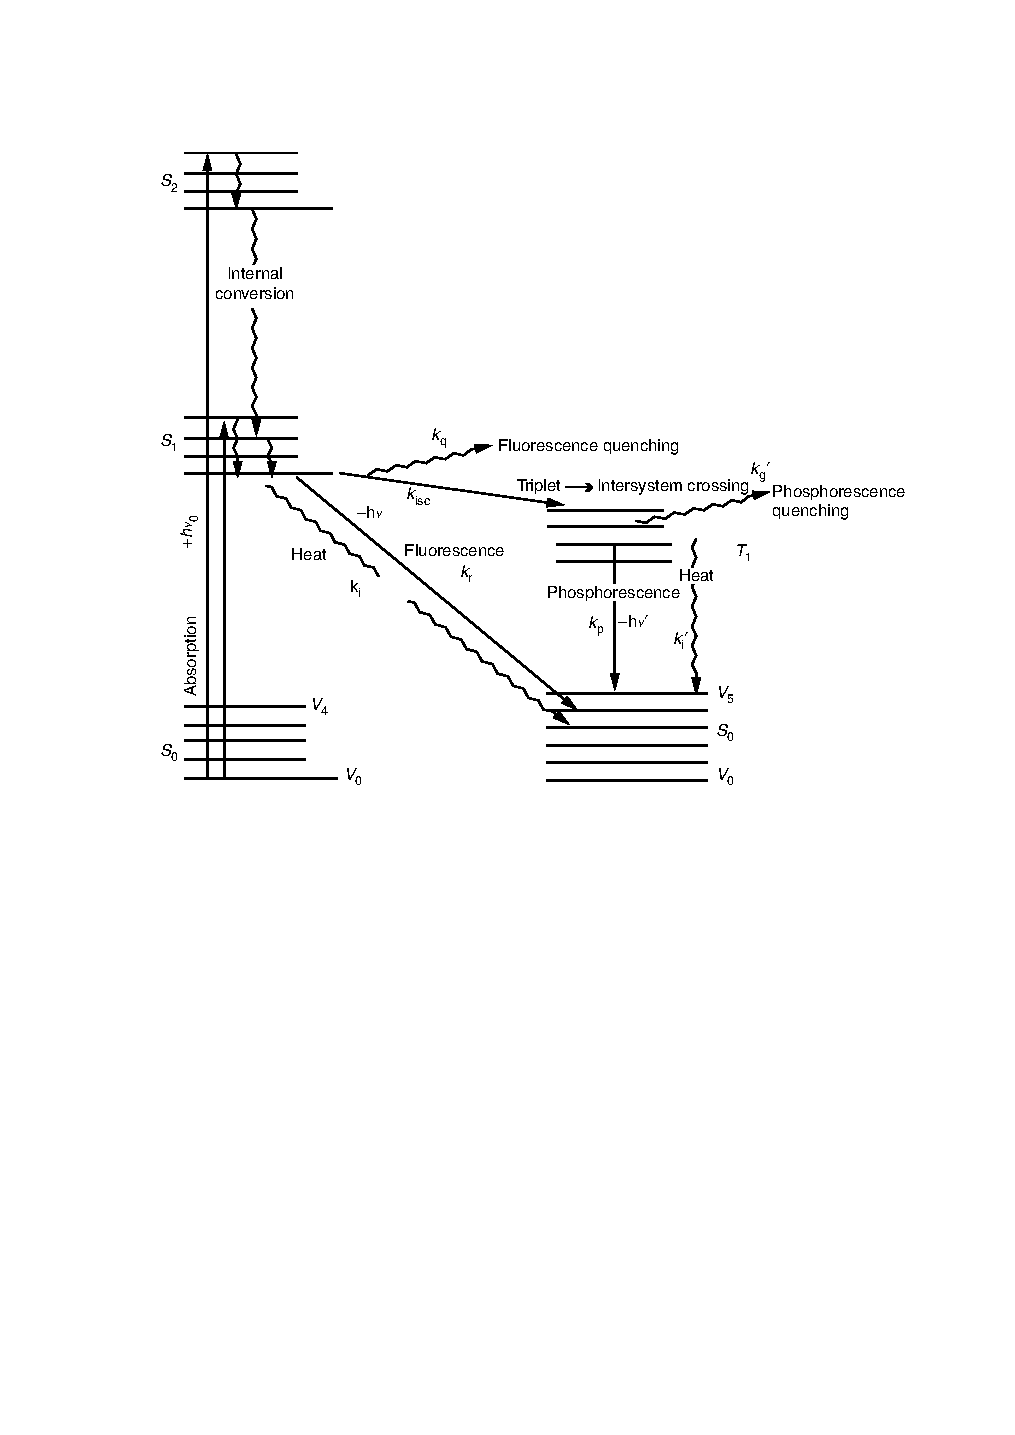
\includegraphics[width=0.87\textwidth]{Figs/fluorescencetrans.pdf}}
	\caption{نمودار یابلونسکی گذارهای الکترونی. نقل از مرجع~\cite{albani2008principles}.}\label{fig:2}
\end{figure}

بازده کوانتمی\LTRfootnote{quantum yield} فرایند فلورسانس را به این صورت تعریف می‌کنند،
\begin{equation}
\Phi=\frac{\text{تعداد فوتون تابش شده}}{\text{تعداد فوتون جذب شده}}.
\end{equation}
از دید دیگر می‌توان بازده را به صورت احتمال تابش فوتون در نظر گرفت و به صورت زیر تعریف کرد،
\begin{equation}
\Phi=\frac{\kappa_r}{\sum \kappa}.
\end{equation}
جمع مخرج روی تمام نرخ‌های فرو افت چه تابشی و چه غیر تابشی انجام می‌پذیرد.

%\section{کاربردهای فلورسانس}
%\subsection{پزشکی}
%\subsection{دیودهای نوری}
%
%\section{ضرورت بهبود تابش فلورسانس}

\section{پلاسمون-پولاریتون‌های سطحی}
پلاسمون‌های سطحی، مطابق تعریف، كوانتم‌های نوسانات چگالی بار سطحی در مرز مشترک فلز-دی‌الکتریک هستند.\footnote{ برخی مراجع، گاهی با قدری تسامح، عبارت پلاسمون سطحی را برای کل مجموعه جفت شده میدان و نوسان بار به کار می‌برند. در این‌جا ما عبارت را به شکل فوق بر اساس تعریف \lr{Novotny} در~\cite{navotny2012} آورده‌ایم.} این نوسانات می‌توانند با میدان‌های الکترومغناطیس روی مرز مشترک جفت شوند و پلاسمون-پولاریتون‌های سطحی \LTRfootnote{surface plasmon polaritons} (\lr{SPP}ها) را تشکیل دهند. از دیدگاه کلاسیک پلاسمون-پولاریتون‌های سطحی جواب‌های خاصی برای معادلات ماکسول تحت شرایط مرزی مشخص به صورت مدهای سطحی می‌باشند.

فرض کنیم که موجی با قطبش $p$ (میدان مغناطیسی موازی سطح) به فصل مشترک دو محیط با توابع دی‌الکتریک $\varepsilon_1(\omega)$ و $\varepsilon_2(\omega)$ مطابق شکل \ref{fig:1} برخورد می‌کند. (می‌دانیم که قطبش $s$ یعنی میدان الکتریکی موازی سطح تولید پلاسمون سطحی نمی‌کند.) ما در پی جواب‌های محدود به فصل مشترک برای معادله موج همگن (بدون برانگیزش خارجی) زیر هستیم.
\begin{align}
&\nabla\times\nabla\times\vec{E}(\vec{r},\omega)-\frac{\omega ^2}{c^2}\varepsilon(\vec{r},\omega)\vec{E}(\vec{r},\omega)=0,\label{eq:2}\\
&\varepsilon(\vec{r},\omega)=\begin{cases}\varepsilon_1(\omega)& z<0,\\
\varepsilon_2(\omega)& z>0.\end{cases}\label{eq:3}
\end{align}
\begin{figure}[tb]
	\centering{
		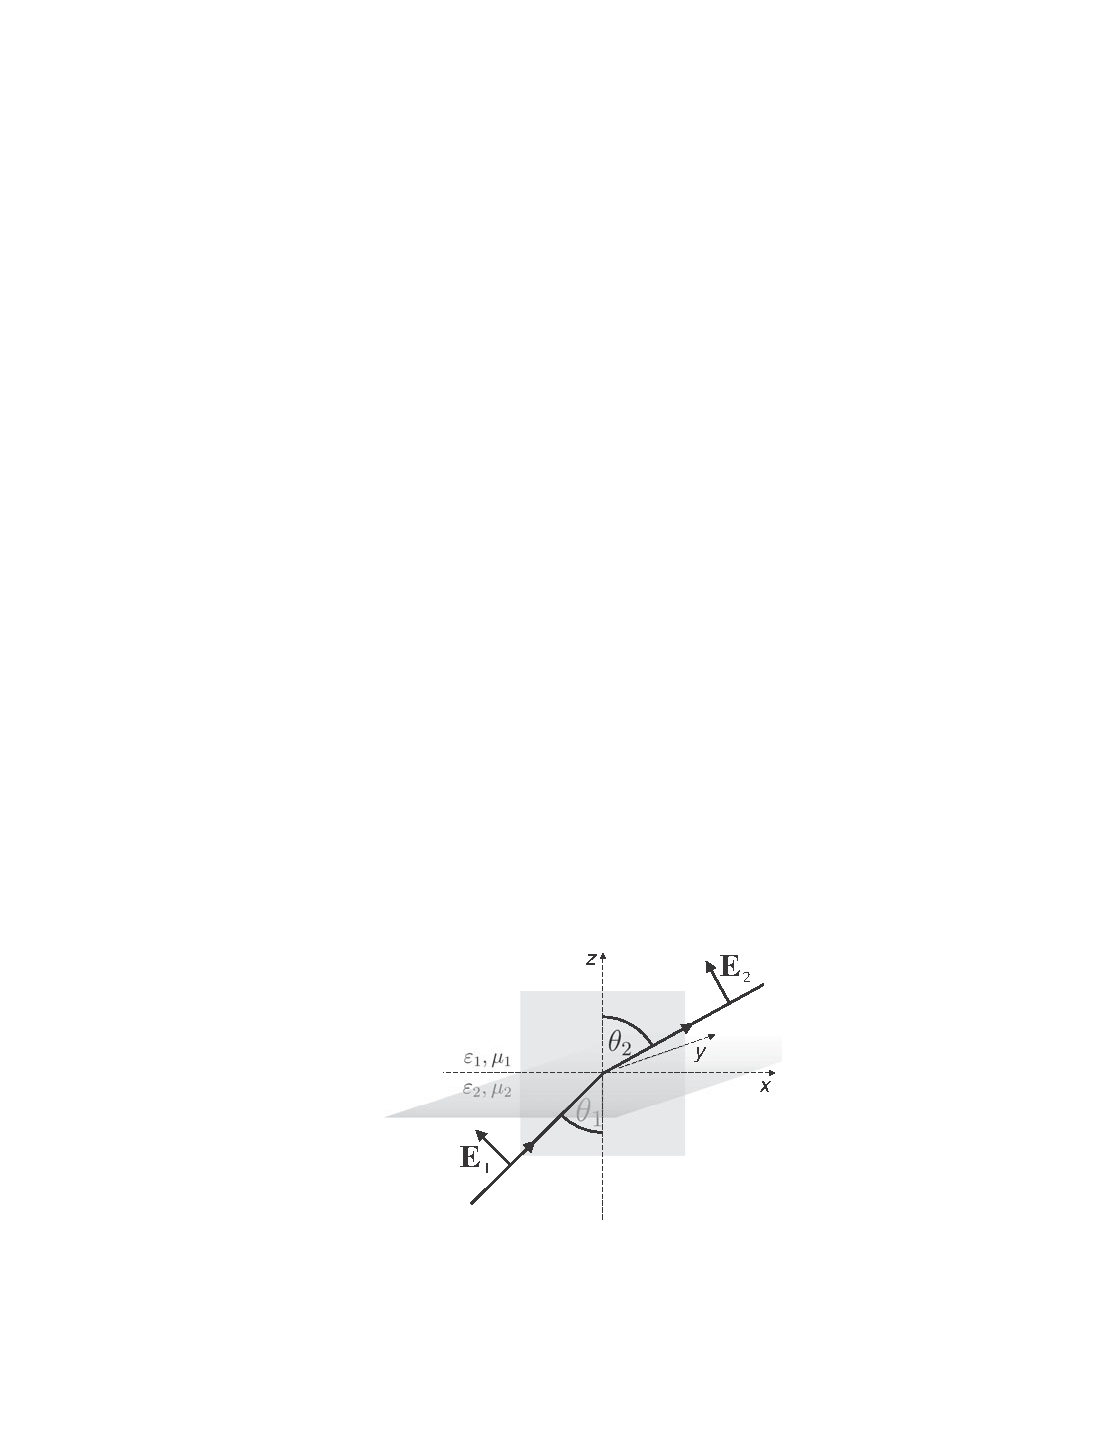
\includegraphics[width=0.5\textwidth]{Figs/incidentwave.pdf}}
	\caption{نمای فصل مشترک دو محیط و موجی با قطبش $p$}\label{fig:1}
\end{figure}

فرم کلی میدان الکتریکی برای قطبش $p$ به صورت زیر می‌تواند باشد.
\begin{equation}\label{eq:4}
\vec{E}_j=\begin{pmatrix}
E_{jx}\\ 0\\ E_{jz}\end{pmatrix}\exp(ik_xx-i\omega t)\exp(ik_{jz}z),\quad j=1,2
\end{equation}
مؤلّفه موازی سطح بردار موج دو طرف مرز برابر است و بین مؤلفه‌ها رابطه زیر برقرار است.
\begin{equation}\label{eq:5}
k_x^2+k_{jz}^2=\varepsilon_jk^2 ,\quad k=2\pi /\lambda.
\end{equation}
همچنین با توجه به عدم وجود بار خارجی، $\nabla .\vec{D}=0$ پس
\begin{equation}\label{eq:6}
k_xE_{jx}+k_{jz}E_{jz}=0.
\end{equation}
بنا بر این بردار میدان الکتریکی در هر محیط را می‌توان به صورت زیر نوشت
\begin{equation}\label{eq:7}
\vec{E}_j=E_{jx}\begin{pmatrix}1\\ 0\\ -k_x/k_{jz}\end{pmatrix}\exp(ik_xx-i\omega t)\exp(ik_{jz}z).
\end{equation}
از طرفی با توجه به شرائط مرزی داریم
\begin{align}
\vec{E}_1^\parallel -\vec{E}_2^\parallel =0\Rightarrow\quad &E_{1x}-E_{2x}=0,\label{eq:8}\\
\vec{D}_1^\perp -\vec{D}_2^\perp =0\Rightarrow\quad &\varepsilon_1E_{1z}-\varepsilon_2E_{2z}=0.\label{eq:9}
\end{align}
این دو معادله به علاوه دو معادله \ref{eq:6} یک دستگاه معادلات برای چهار مؤلفه مجهول میدان می‌سازند و شرط جواب داشتن دستگاه (صفر شدن دترمینان ضرائب) در دو حالت اتفاق می‌افتد: یکی این که $k_x=0$ یعنی هیچ انتشار موازی سطحی وجود ندارد که مطلوب نیست و دیگری این که
\begin{equation}\label{eq:10}
\varepsilon_1k_{2z}-\varepsilon_1k_{1z}=0.
\end{equation}
ابن رابطه به همراه معادله \ref{eq:5} رابطه پاشندگی به دست می‌دهد؛ یعنی رابطه‌ای میان بردار موج در راستای انتشار (موازی سطح) و فرکانس زاویه‌ای $\omega$،
\begin{equation}\label{eq:11}
k_x^2=\frac{\varepsilon_1\varepsilon_2}{\varepsilon_1+\varepsilon_2}k^2=\frac{\varepsilon_1\varepsilon_2}{\varepsilon_1+\varepsilon_2}\frac{\omega^2}{c^2}.
\end{equation}
همچنین رابطه‌ای برای مؤلفه عمود بر سطح بردار موج خواهیم داشت
\begin{equation}\label{eq:12}
k_{jz}^2=\frac{\varepsilon_j^2}{\varepsilon_1+\varepsilon_2}k^2.
\end{equation}
اکنون می‌توان از شرائط لازم برای وجود مدهای سطحی (مدی که روی فصل مشترک منتشر شود) سخن گفت. وجود این مدها معادل یافتن $k_x$ حقیقی (یا دارای جزء حقیقی) است. بنا بر این باید صورت و مخرج کسر معادله \ref{eq:11} یعنی $\varepsilon_1\varepsilon_2$ و $\varepsilon_1+\varepsilon_2$ هم علامت باشند. علاوه بر این مدها باید محدود به سطح باشند پس در راستای عمود بر سطح نباید منتشر شوند و عدد موج  در این راستا یعنی $k_{jz}$ باید موهومی شود و این تنها با منفی شدن مخرج کسر معادله \ref{eq:12} یعنی $\varepsilon_1+\varepsilon_2$ امکان‌پذیر است. در مجموع شرط وجود مدهای سطحی این است که
\begin{eqnarray}
\varepsilon_1(\omega).\varepsilon_2(\omega)&<0,\label{eq:13}\\
\varepsilon_1(\omega)+\varepsilon_2(\omega)&<0,\label{eq:14}
\end{eqnarray}
یعنی قسمت حقیقی تابع دی‌الکتریک یکی از محیط‌ها باید منفی باشد و همچنین قدر مطلق آن باید از قسمت حقیقی تابع دی‌الکتریک محیط دیگر بیشتر باشد.

همان‌گونه که می‌دانیم، فلزها، مخصوصًا فلزهای کمیاب مانند طلا و نقره، تابع دی‌الکتریکی با قسمت حقیقی منفی و قسمت موهومی بسیار کوچک دارند و می‌توان این مدهای سطحی را که پلاسمون-پولاریتون‌هایسطحی (به اختصار \lr{SPP}) می‌نامیمشان، در فصل مشترک فلز-دی‌الکتریک ایجاد کرد.
تابع دی‌الکتریک فلزات از دو بخش حقیقی و موهومی تشکیل شده
\begin{equation}\label{eq_1}
\varepsilon(\omega)=\varepsilon ^\prime (\omega) +i\varepsilon ^{\prime\prime}(\omega)
\end{equation}
که در فرکانس‌های اپتیکی، برای فلزات کمیاب معمولًا $|\varepsilon ^\prime |>|\varepsilon ^{\prime\prime }|$ است.
مختلط بودن تابع دی‌الکتریک منجر به مختلط شدن مؤلفه موازی سطح بردار موج می‌شود؛ یعنی $k_x=k_x^\prime+ik_x^{\prime\prime}$ که با در نظر گرفتن $|\varepsilon_1^{\prime\prime}|\ll |\varepsilon_1^\prime|$ و حقیقی فرض کردن $\varepsilon_2$ از معادله \ref{eq:11} خواهیم داشت
\begin{eqnarray}
k_x^\prime\approx\frac{\omega}{c}\sqrt{\frac{\varepsilon_1^\prime\varepsilon_2}{\varepsilon_1^\prime+\varepsilon_2}},\label{eq:15}\\
k_x^{\prime\prime}\approx\frac{\omega}{c}\frac{\varepsilon_1^{\prime\prime}\varepsilon_2}{2\varepsilon_1^\prime(\varepsilon_1^\prime+\varepsilon_2)}\sqrt{\frac{\varepsilon_1^\prime\varepsilon_2}{\varepsilon_1^\prime+\varepsilon_2}}.\label{eq:16}
\end{eqnarray}

می‌توان برای امواج منتشر‌شونده موازی سطح یک طول موج با عنوان طول‌موج پلاسمون به صورت زیر در نظر گرفت .
\begin{equation}\label{eq:17}
\lambda_\text{SPP}=\frac{2\pi}{k_x^\prime}\approx\lambda\sqrt{\frac{\varepsilon_1^\prime+\varepsilon_2}{\varepsilon_1^\prime\varepsilon_2}}
\end{equation}

طول انتشار پلاسمون:\\
جزء موهومی $k_x$ موجب میرایی موج منتشر شده موازی سطح می‌شود. بنا بر این می‌توان $1/k_x^{\prime\prime}$ را به عنوان مقیاسی از طول انتشار پلاسمون در نظر گرفت. میدان موج پلاسمون سطحی پس از طی این طول به $1/\mathbf{e}$ مقدار ماکزیمم خود کاهش می‌یابد.

امواج ناپایای پلاسمون:\\
با مختلط شدن $\varepsilon_1$، مؤلفه عمود بر سطح بردار موج در هر محیط، $k_{jz}$، مختلط می‌شود و در نتیجه امواج در راستای عمود بر سطح میرا می‌گردند.
\begin{eqnarray}
k_{1z}=\frac{\omega}{c}\sqrt{\frac{\varepsilon_1^{\prime 2}}{\varepsilon_1^\prime+\varepsilon_2}}\left[1+i\frac{\varepsilon_1^{\prime\prime}}{2\varepsilon_1^\prime}\right],\label{eq:18}\\
k_{2z}=\frac{\omega}{c}\sqrt{\frac{\varepsilon_2^2}{\varepsilon_1^\prime+\varepsilon_2}}\left[1-i\frac{\varepsilon_1^{\prime\prime}}{2\left(\varepsilon_1^\prime+\varepsilon_2\right)}\right],\label{eq:19}
\end{eqnarray}
به عبارت دیگر در راستای عمود بر سطح \emph{موج ناپایا}\LTRfootnote{evanescent wave} خواهیم داشت. طول میرایی این امواج نیز با مقیاس $1/k_{jz}$ سنجیده می‌شود.

\section{تحقیقات پیشین}
\begin{figure}[tb]%[tbh]
	\centering{
		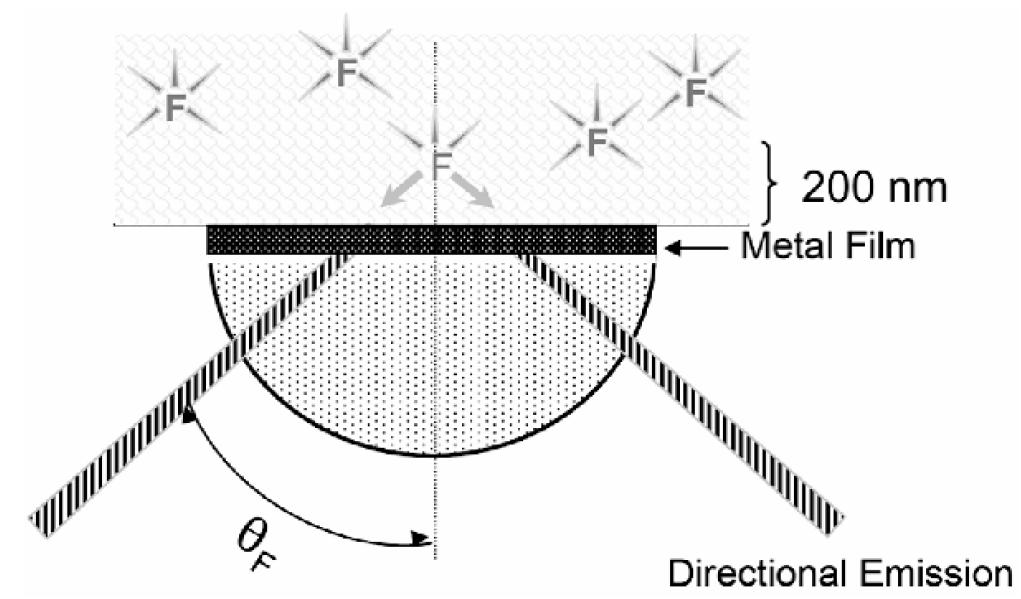
\includegraphics[width=.7\textwidth]{Figs/directionalemission.jpg}}
	\caption{نمایشی از \lr{SPCE}. حرف \lr{F} نشانگر فلوروفور است. نقل از مرجع~\cite{calander2004theory}.}\label{fig:3}
\end{figure}
اگر در نزدیکی فصل مشترک فلز-دی‌الکتریک، یک مولکول برانگیخته فلوروفور\LTRfootnote{fluorophore} قرار بگیرد، تابش فلورسانس حاصل می‌تواند پلاسمون‌های سطحی را تحریک کند و امواج پلاریتون پلاسمون سطحی در همان فرکانسِ تابش فلورسانس نوسان کنند. از سوی دیگر، همان‌گونه که گفته شد، پلاسمون سطحی میدان ناپایایی در مجاورت فصل مشترک فلز-دی‌الکتریک ایجاد می‌کند و شدت در نزدیکی سطح فلز بسیار افزایش می‌یابد. اگر یک مولکول فلوروفور در این میدان ناپایا قرار گیرد، برانگیخته می‌شود و با احتمالی متناسب با $\kappa_r$ تابش می‌کند. این برهمکنش متقابل به تابش کوپل شده پلاسمون سطحی \lr{(SPCE)}\LTRfootnote{Surface Plasmon Coupled Emission} شناخته می‌شود. \lr{Calander} و همکاران~\cite{calander2004theory} و همچنین گروه \lr{Knoll}~\cite{ekgasit2004evanescent,vasilev2004fluorescence} با رویکردی تئوری نشان داده‌اند این برهمکنش در مجاورت سطوح تخت فلزی با لایه نازک دی‌الکتریک منجر به تابشی بسیار جهتمند می‌شود. 

این جهتمند شدن تابش فلورسانس، که ذاتًا از نوع تابش خودبه‌خودی\LTRfootnote{spontaneous emission} و کاتوره است، ناشی از جفت‌شدگی نوسانات بارهای سطح فلز و نوسانات دو قطبی مولکول فلورسانس (تقریب دو قطبی مولکول برانگیخته) دانسته شده است.


علاوه بر این، نزدیکی ذرات فلز و مولکول فلورفور منجر به افزایش شدت تابش فلورسانس، افزایش پایداری نوری\LTRfootnote{photostability} و افزایش فاصله انتقال انرژی نوسانس فلورسانس (\lr{FRET})\LTRfootnote{fluorescence resonance energy transfer} می‌گردد~\cite{Selvin2000} که به مجموعه این پدیده‌ها فلورسانس افزایش یافته با فلز (\lr{MEF})\LTRfootnote{metal-enhanced fluorecsence} می‌گویند~\cite{ribeiro2017artefact}.

افزایش دامنه این تحقیقات، شاخه کلی‌تری در دانش پلاسمونیک و فلورسانس به نام فلورسانس کنترل شده با پلاسمون (\lr{PCF})\LTRfootnote{plasmon-controlled fluorescence}~\cite{doi:10.1021/jz201392k,B802918K} به‌وجود آورده است. در این حوزه تحقیقات، علاوه بر موارد فوق، با توجه به این‌که نزدیکی فلوروفور و نانو ذره فلزی منجر به انتفال انرژی از فلوروفور برانگیخته به نانو ذره می‌شود، امکان کنترل نرخ فرو افت غیرتابشی فراهم می‌شود و با تنظیم فاصله و اندازه و شکل نانو ذرات فلزی، نرخ فرو افت غیرتابشی و تابشی (بوسیله پلاسمون سطحی) را مهندسی می‌کنند(\lr{RDE})\LTRfootnote{radiative decay engineering}~\cite{gryczynski2004radiative,geddes2007radiative} که نتیجه آن، بازده کوانتمیِ فلورسانسِ قابل تنظیم است.


\begin{figure}[tb]
	\centering{
		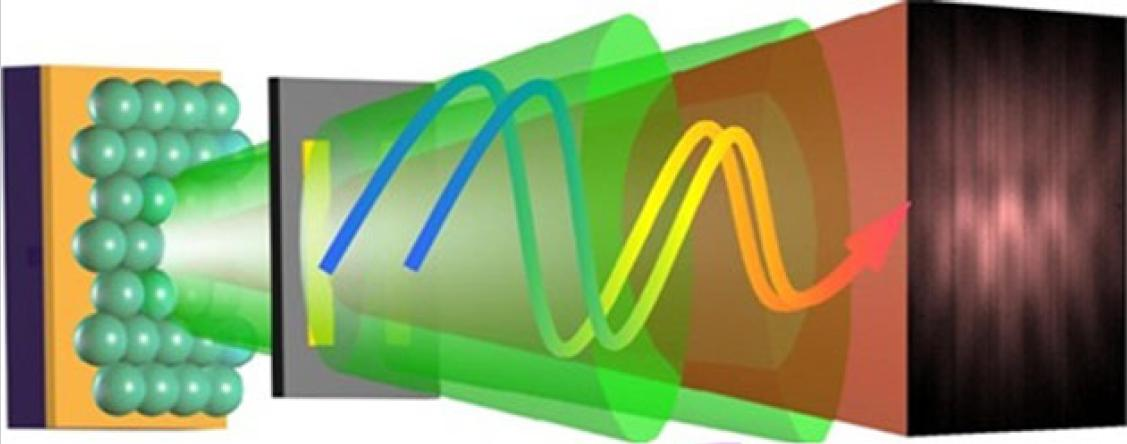
\includegraphics[width=.65\textwidth]{Figs/coherent.jpg}}
	\caption{نمایشی از تأثیر ساختار بلور دوگانه پلاسمونیک(لایه فلزی سمت چپ)-فوتونیک(آرایه کره‌های دی‌الکتریک) بر همدوسی تابش فلورسانس. نقل از مرجع~\cite{shi2014coherent}.\label{fig3_1}}
\end{figure}

اخیرًا تحقیقی بر همدوس کردن تابش فلورسانس انجام شده است~\cite{shi2014coherent}. در این تحقیق، در مجاورت یک ساختار بلور فتونیک-پلاسمونیک فلوروفور قرار داده می‌شود و به کمک پلاسمون‌های سطحی و مدهای هدایت شده دی‌الکتریک درجه‌ای از همدوسی در تابش ایجاد می‌شود. طول همدوسی فضایی حدود 10 برابر طول‌موج تابش و همدوسی زمانی حدود 4 برابر زمان همدوسی تابش فلورسانس اندازگیری شده است.

\begin{figure}[tb]
	\centering{
		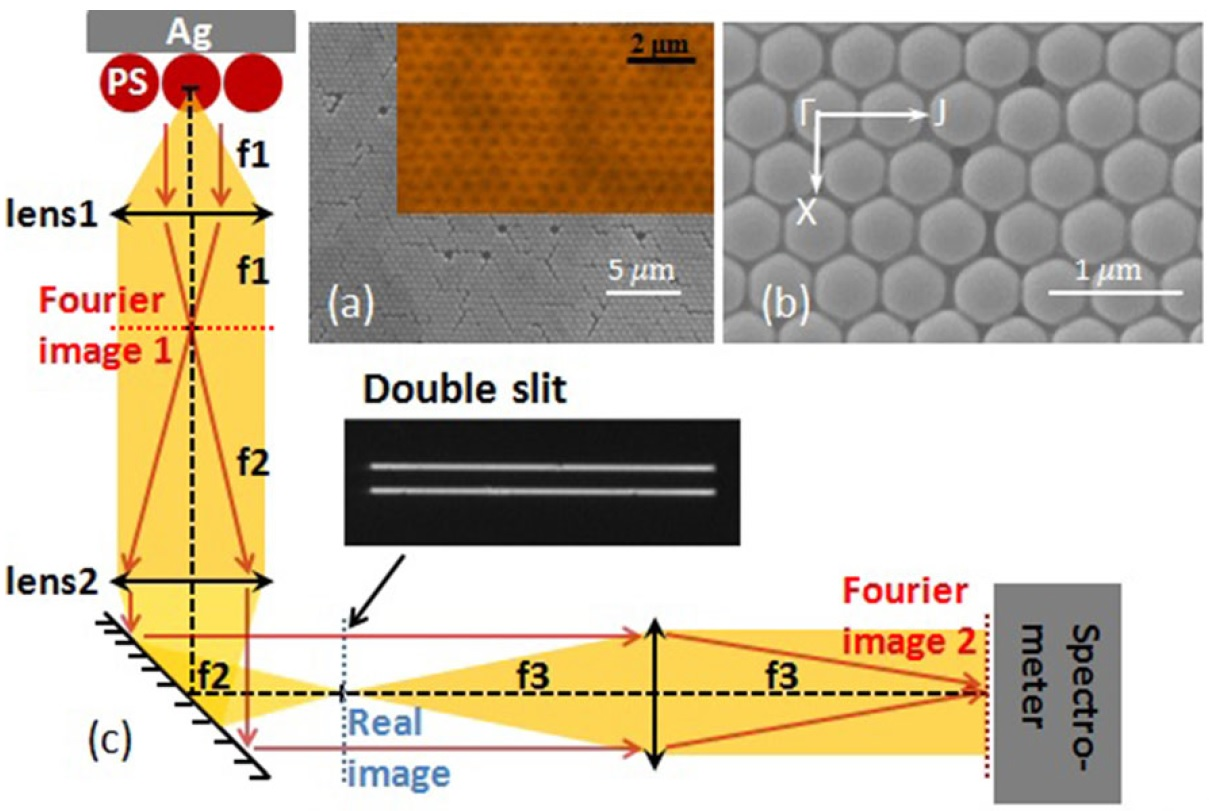
\includegraphics[width=.8\textwidth]{Figs/coherent_setup.jpg}}
	\caption{تصویر ساختار بلور دوگانه حاصل از \lr{SEM} با بزرگنمایی‌های مختلف به همراه نمایشی از چینش آزمایش تجربی همدوسی فلورسانس. نقل از مرجع~\cite{shi2014coherent}.}\label{fig3_1}
\end{figure}


بلورهای فوتونیک\LTRfootnote{photonic crystals} ساختارهایی با تغییرات تناوبی ضریب‌شکست هستند که می‌توانند به صورت‌های یک‌بعدی تا سه‌بعدی ایجاد شوند. بلور دوگانه فوتونیک-پلاسمونیک\LTRfootnote{photonic-plasmonic crystal} از آرایه‌ای از نانو ذرات دی‌الکتریک بر روی لایه نازک فلز ایجاد می‌شود~\cite{romanov2011}. این آرایه می‌تواند ساختار دوبعدی یا سه‌بعدی داشته باشد. این آرایه توسط یک لایه نازک دی‌الکتریک از لایه فلزی جدا می‌گردد. لایه نازک فلزی نیز می‌تواند به صورت تخت یا حتی شیاردار\LTRfootnote{corrugated} باشد.
\begin{figure}[tb]
	\centering{
		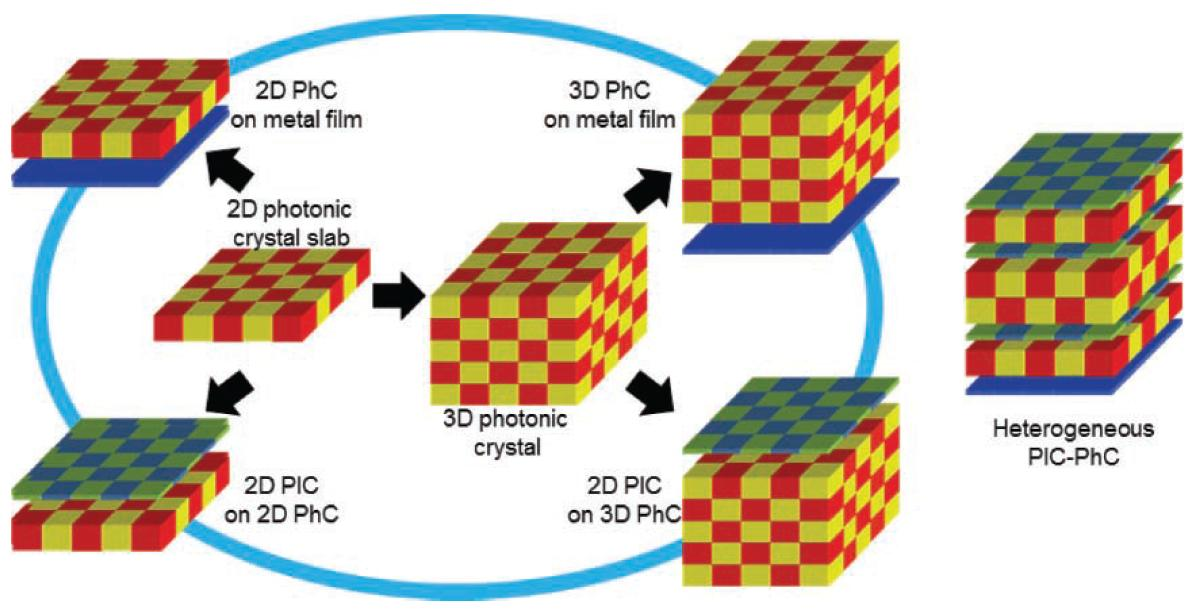
\includegraphics[width=0.8\textwidth]{Figs/hybrid.jpg}}
	\caption{نمای شماتیک از نمونه‌های مختلفی از ساختار بلور دوگانه فوتونیک-پلاسمونیک. \lr{PhC} نشانگر بلور فوتونی و \lr{PlC} نشانگر بلور پلاسمونیک(لایه شیارداری از فلز) می‌باشد. نقل از مرجع~\cite{romanov2011}.}\label{fig:4}
\end{figure}
\begin{figure}[tb]
\centering{
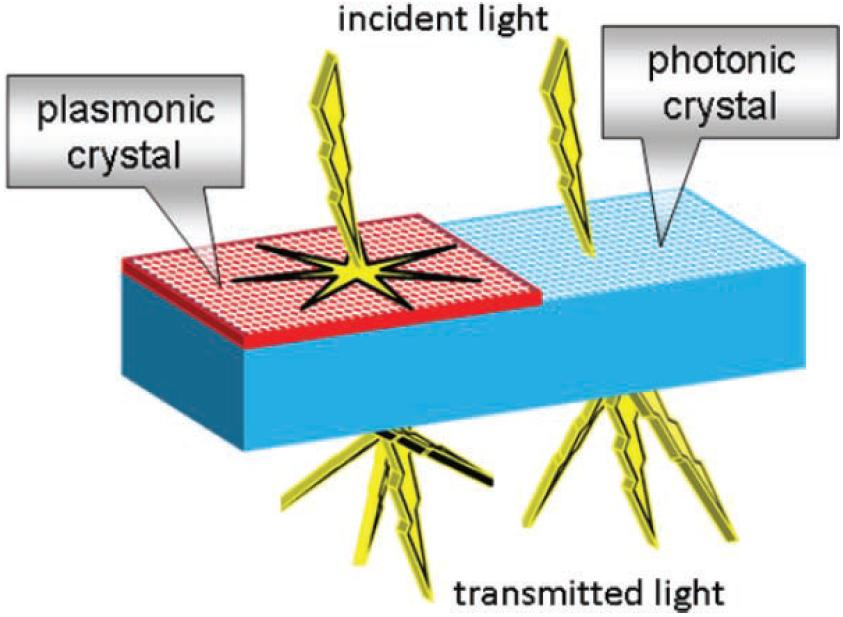
\includegraphics[width=.4\textwidth]{Figs/PlC_PhC.jpg}}
\caption{نمایشی از یک ساختار دوگانه پلاسمونیک-فوتونیک. نقل از مرجع~\cite{romanov2011}.}\label{fig4_1}
\end{figure}

\begin{figure}[tb]
	\centering{
		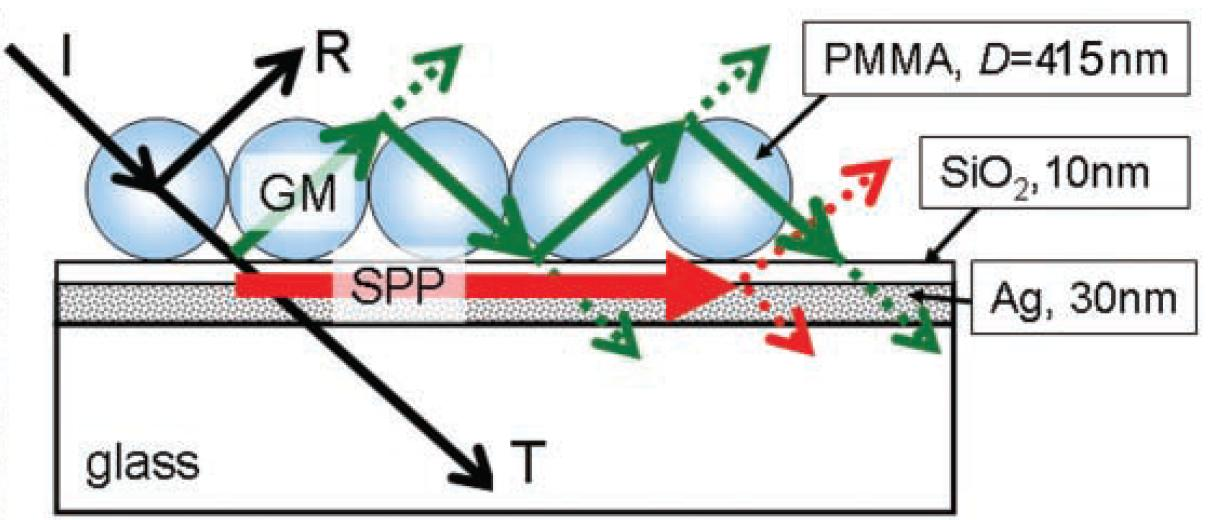
\includegraphics[width=.7\textwidth]{Figs/hybrid2.jpg}}
	\caption{انتشار موج در ساختار بلور دوگانه. پرتو فرودی(\lr{I}) به پرتوهای بازتابی(\lr{R}) و عبوری(\lr{T}) تفکیک می‌شود و در عین حال هم مدهایی درون کره‌ها هدایت می‌شود و هم پلاسمون سطحی تحریک شده و منتشر می‌‌گردد. پرتوهای خط‌چین اتلاف‌ها را نشان می‌دهد. نقل از مرجع~\cite{SHI20101059}.}\label{fig4_2}
\end{figure}
\begin{figure}[tb]
	\centering{
		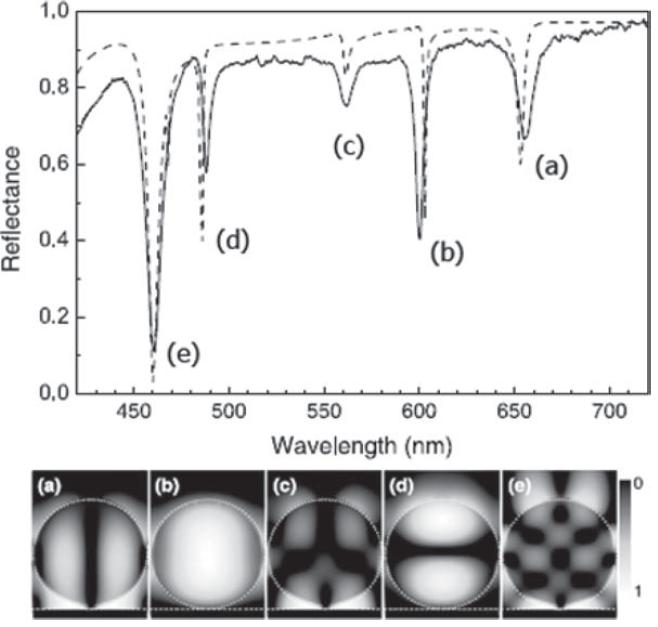
\includegraphics[width=0.6\textwidth]{Figs/reflection.jpg}}
	\caption{نمودار بازتاب اندازگیری شده (خط ممتد) و شبیه‌سازی شده (خط‌چین) برای آرایه‌ای از کره‌های پلی‌استر با قطر $500nm$ که با لایه‌ای از $SiO_2$ به ضخامت $5nm$ از لایه بستر نقره با ضخامت $200nm$ جدا شده است. جهت تابش عمود بر لایه است. در قسمت پایین نوسان مدهای عبوری در یک کره پلی‌استر (دایره خط‌چین) روی بستر نقره (خط‌چین زیر) برای مدهای عبوری مشخص شده روی نمودار بالا نمایش داده شده است. نقل از مرجع~\cite{SHI20101059}.}\label{fig:5}
\end{figure}

این ساختارها مدهای عبوری ویژه‌ای دارند (شکل \ref{fig4_2}) و در طول‌موج‌های خاصی بازتاب بسیار کم و عبور زیاد می‌شود. به طور نمونه، شکل \ref{fig:5} نتیجه تحقیقی توسط \lr{Shi} و همکاران است که نمودار بازتاب یکی ساختار خاص را نشان می‌دهد~\cite{SHI20101059}. با هماهنگ کردن این مدهای عبوری و طول‌موج تابش فلورسانس می‌توان به همدوسی تابش فلورسانس دست یافت~\cite{shi2014coherent}.

به بیان  دقیق‌تر، مدهای هدایت شده درون شبكه فوتونی با مولكول‌های فلوروفور برهمكنش میكنند و جفت‌شدگی آنها موجب تابش هماهنگ و همدوس می‌‌شود. از طرف دیگر این شبكه همانند یك توری پراش موحب تحریك مدهای پلاسمون سطحی فلز می‌شود و انتشار \lr{SPP}ها موازی سطح تابش مولكول‌ها را به هم مرتبط می‌نماید. هر چه طول انتشار \lr{SPP}ها بیشتر باشد نه تنها مولكول‌های مجاور بلكه مولكول‌های دور دست نیز جفت می‌شوند و همدوسی تابش خروجی افزایش مییابد.

\section{شبیه‌سازی عددی}
با در نظر گرفتن محدودیت‌هایی که در راه تحقیقات عملی آزمایشگاهی است، روش‌های شبیه‌سازی عددی با هزینه کمتر، نه  تنها می‌توانند در برپایی یک چینش دقیق آزمایشگاهی و رسیدن به نمونه مطلوب راهنما باشند~\cite{Bradford:14,Lee:18}، بلکه می‌توانند دید فیزیکی ما از چگونگی روی‌داد یک پدیده را ارتقاء دهند~\cite{cao2000transition,PhysRevE.98.063304}.

در موضوع مورد بحث این تحقیق، پیچیدگی‌هایی  در مسأله وجود دارد. مولکول‌های تابشگر علاوه‌بر این‌که با میدان خارجی اعمال شده برهم‌کنش دارند، از میدان تابش‌شده توسط سایر مولکول‌ها نیز تأثیر 
می‌پذیرند. به عیارت دیگر علاوه‌بر برهم‌کنش با عامل خارجی، سیستم حاوی برهم‌کنش‌های داخلی نیز هست که این برهم‌کنش‌های داخلی می‌توانند کوتاه برد باشند و تنها در میان مولکول‌های همسایه، و یا می‌توانند با مدهای هدایت‌شده فوتونی یا پلاسمونی، مولکول‌های دوردست نیز برهمکنش‌های بلندبرد داشته باشند. بنا بر این، ما با یک سیستم بس‌ذره‌ای از تابشگرها مواجهیم که انواع برهم‌کنش‌های خارجی و داخلی در آن وجود دارد. می‌توان پیش‌بینی کرد که این سیستم خواص آماری جالب توجهی مانند همدوسی ویا حتّی گذار فاز را بروز دهد. پس لازم است روش شبیه‌سازی این سیستم این قابلیت را داشته باشد که با منظور کردن رفتار میکروسکوپی اجزاء، خواص آماری جمعی آن‌ها را نیز به دست بدهد.

اغلب روش‌هایی که تا کنون برای شبیه‌سازی مولکول‌های فلورسانس به کار رفته‌اند بر پایه معادلات جبرگرایانه\footnote{کلمه \emph{جبرگرایانه} به عنوان معادل واژه \lr{deterministic} استفاده شده است. به عنوان معادل‌های دیگر این عبارت، گاهی معادلات \it{حتمی} یا \emph{تَعَیُّنی} نیز به دلیل قابل تعیین بودن رفتار و حتمی بودن نتیجه، به‌کار می‌رود امّا هیچ‌کدام مجبور بودن سیستم به بروز رفتار مشخص را به چشم خواننده نمی‌آورد. بنا بر این، صرف‌نظر از بار فلسفی همراه عبارت \emph{جبرگرایانه}، در این رساله از همین کلمه استفاده کرده‌ایم. } بنا شده‌اند. به عبارت دیگر، دو مولکول مستقل، زمانی که در شرائط مشابهی قرار دارند دقیقًا یک رفتار را نشان می‌دهند. از سوی دیگر رفتار جمعی آماری زمانی که تمام اجزاء، در شرائط مشابه، رفتاری کاملًا یکسان بروز دهند معنای فیزیکی خود را از دست می‌دهد. بنا بر این لازم است که طبیعت احتمالاتی گذارهای مولکولی در محاسبات منظور شود.

به طور کلی روش‌های عددی شبیه‌سازی تابشگرها را می‌توان در دو گروه دسته‌بندی کرد:
\begin{enumerate}[label=(\alph*)]
	\item روش‌هایی که برپایه دیدگاه \emph{ماکروسکوپی} بنا شده‌اند؛ یعنی  اساسًا از کمیّت‌هایی استفاده می‌کنند که از میانگین‌گیری آماری حاصل شده‌اند. به عنوان نمونه، استفاده از ضرائب مؤثر اپتیکی مثل ضریب‌گذردهی یا ضریب رسانایی~\cite{cao2000transition,7769917} و یا استفاده از چگالی جمعیّت ترازهای انرژی~\cite{Chang:04,662652,PhysRevA.52.3082}.
	\item روش‌هایی که برپایه دیدگاه \emph{میکروسکوپی} بنا شده‌اند؛ یعنی رفتار تک‌مولکول را مورد تمرکز قرار می‌دهند. به عنوان نمونه، موارد متعددی که مولکول را به صورت کلاسیکی یک دوقطبی در حال نوسان در نظر می‌گیرند~\cite{PhysRevLett.95.013904,genevet2010large,wang2011optical,bauch2013collective,Hoang2015,javadi2018numerical} و یا مواردی که با دیدگاه مکانیک کوانتمی معادله شرودینگر یا معادلات توابع چگالی را حل می‌کنند~\cite{PhysRevB.82.075427,PhysRevA.45.4879,Hong_2015,doi:10.1021/jp1043392}.
\end{enumerate}

دیدگاه ماکروسکوپی در شبیه‌سازی توده پیوسته مواد فعال (مانند محیط بهره لیزر) عمل‌کرد بسیار خوبی دارد. اما این دسته روش‌ها، رفتار جمعی تعداد زیادی تابشگر که در شرائط یکسانی قرار دارند به وسیله کمیت‌های میانگین‌گیری شده نشان داده مي‌شود. بنا بر این، این روش‌ها انتخاب مناسبی برای مسائلی که تعداد زیادی تابشگر با جهت‌گیری‌های متفاوت راستای مولکول و یا در حضور ناهمگنی‌‌های محیطی متغیر با زمان قرار دارند نمی‌باشد. علاوه‌بر این‌ها، معادلات جبرگرایانه حاکم بر این روش‌ها هم ماهیت احتمالاتی تابش خود‌به‌خودی را نادیده می‌گیرند.

از سوی دیگر روش‌هایی که با دیدگاه میکروسکوپی و روی‌کرد کوانتمی عمل می‌کنند، لازم است با محاسبات سنگین عددی، معادلاتی مانند شرودینگر با حضور جملاتی که برهم‌کنش‌های تابشگر-میدان خارجی و تابشگر-تابشگر حل شوند~\cite{doi:10.1021/jp1043392}. این گونه محاسبات معمولًا برای تعداد معدودی تابشگر قابل انجام هستند. گاهی با یکسان در نظر گرفتن تمام تابشگرها و فرض یکنواختی محیط، مسأله بس-تابشگر را با دیدگاه کوانتمی حل می‌کنند~\cite{PhysRevB.91.035306} اما در شرائ غیر یکنواخت گزینه مناسبی نیست.

مواردی که در دیدگاه میکروسکوپی مولکول‌ها را با روی‌کرد کلاسیکی با دوقطبی‌های در حال نوسان مدل می‌کنند، بسیار متعددند. مخصوصًا این روش قابلیّت بسیار خوبی برای جفت شدن با روش‌های عددی شبیه‌سازی انتشار امواج در دامنه زمانی (مانند \lr{FDTD}) دارند و زیاد در تحقیقات به کار رفته‌اند. اما در این روش، فرکانس جذب و تابش مولکول یکسان در نظر گرفته می‌شود و به عبارتی تنها مدل دوترازه تابشگر شبیه‌سازی می‌شود~\cite{Witthaut_2010,PhysRevLett.106.053601}. نقص مهم‌تر اما این است که در نظر گرفتن یک معادله دیفرانسیل یکسان برای تمام تابشگرها منجر به رفتار جبری و یکسان همه آنها در شرائط مشابه می‌شود و ماهیت آماری از دست می‌رود.

\section{اهداف رساله}
در این تحقیق، با بررسی برهمکنش فلورسانس-پلاسمون سطحی در چینش‌ها و ساختارهای مختلف، از یک سو سعی در ارائه توجیه و تفسیر فیزیکی برای مشاهدات یافته شده مانند جهتمندی یا همدوسی تابش فلورسانس، و از سوی دیگر تلاش برای بهبود این تابش با ارائه ساختارها و چینش‌های مناسب‌تر، مورد پیگیری خواهد بود. 
به طور نمونه در تحقیقات فعلی تنها حالت خاصی از ترکیب بلور فوتونی و فلز مورد بررسی قرار گرفته است. همچنین ساخت و به کار بردن ساختار بررسی‌شده فعلی (آرایه ذرات روی بستر فلزی) برای حسگر و تصویربرداری فلورسانس (مثلًا برای تزریق به بافت) ممکن است با دشواری‌های فراوانی همراه باشد. بنابر این، این سؤال همچنان باز است که چه چینش‌های دیگری ممکن است به بهبود همدوسی و جهتمندی تابش فلورسانس بیانجامد و برای ساخت و استفاده سهل‌الوصول باشد.

در این مسیر استفاده از روش‌های شبیه‌سازی بسیار می‌تواند به حل مسائل کمک نماید. ارائه روش عددی مناسب برای وارد کردن تابشگرهای خود‌به‌خودی (مانند فلورسانس) در شیوه‌های متداول شبیه‌سازی مانند روش \lr{FDTD} به صورتی که نواقص روش‌هایی که قبلا استفاده شده‌است رفع گردد و بتواند رفتارهای آماری تعداد زیادی تابشگر را با منظور کردن ماهیت احتمالاتی گذارها به دست دهد، از اهداف اصلی پژوهش حاضر است.

در ادامه این رساله، آشنایی مختصر با روش \lr{FDTD}، نحوه اعمال اجزاء آن مانند مرزهای جاذب یا موج فرودی، مدل استفاده شده برای محیط‌های پاشنده و فلزی در این روش و همچنین شیوه کدنویسی و بسته ایجاد شده برای شبیه‌سازی مختصرًا در فصل~\ref{chap2} توضیح داده می‌شود. شرح روش عددی جدیدی که برای شبیه‌سازی تابشگرهای خودبه‌خودی معرفی کرده‌ایم به همراه نمونه‌های شبیه‌سازی شده با هدف محک‌زدن اعتبار روش در فصل~\ref{chap3} ارائه خواهد شد. ساختار دوگانه فوتونی-پلاسمونی پیشنهادی برای بهبود همدوسی تابش فلورسانس و نتائج مربوط به آن، به همراه تحلیل فیزیکی مکانیزم ایجاد همدوسی، در فصل~\ref{chap4} تشریح و حاصل پژوهش در فصل آخر جمع‌بندی خواهد شد.

%از سوی دیگر، قبلًا نشان داده‌ایم که بسیاری از خواص بلور منظم فوتونی، مانند مدهای عبوری، در ساختاری نامنظم نیز پایدار می‌مانند و تنها چگالی توزیع نانو ذرات بر این خواص اثرگذار است؛ حال، با توجه به این‌که ساخت و به‌کاربری یک چینش کاتوره بسیار آسان‌تر است، بررسی تأثیرات بی‌نظمی وکاتورگی در ساختارهای فوتونیک-پلاسمونیک احتمال بهبود جهتمندی و همدوسی و افزایش یافتن تابش فلورسانس و امکان کنترل این تابش می‌تواند راه‌گشا باشد.

%علاوه بر موارد فوق، حضور موادی مانند گرافن -ساختاری با خواص ویژه- می‌تواند اثرات جالب توجهی بر تابش فلورسانس داشته باشد كه بررسی آن بسیار ثمر بخش خواهد بود.